% \documentclass[aspectratio=169,notes]{beamer}
\documentclass[aspectratio=169]{beamer}
\usetheme[faculty=phil]{fibeamer}
\usepackage{polyglossia}
\setmainlanguage{english} %% main locale instead of `english`, you
%% can typeset the presentation in either Czech or Slovak,
%% respectively.
\setotherlanguages{russian} %% The additional keys allow
%%
%%   \begin{otherlanguage}{czech}   ... \end{otherlanguage}
%%   \begin{otherlanguage}{slovak}  ... \end{otherlanguage}
%%
%% These macros specify information about the presentation
\title[IME]{Introduction to Mechanical Engineering, HW CAD ASM 2} %% that will be typeset on the
\subtitle{Complex Assembly
\\ \  \\ \ 
         } %% title page.
\author{Oleg Bulichev}
%% These additional packages are used within the document:
\usepackage{ragged2e}  % `\justifying` text
\usepackage{booktabs}  % Tables
\usepackage{tabularx}
\usepackage{tikz}      % Diagrams
\usetikzlibrary{calc, shapes, backgrounds}
\usepackage{amsmath, amssymb}
\usepackage{url}       % `\url`s
\usepackage{listings}  % Code listings
% \usepackage{subfigure}
\usepackage{floatrow}
\usepackage{subcaption}
\usepackage{mathtools}
\usepackage{todonotes}
\usepackage{fontspec}
\usepackage{multicol}
\usepackage{pdfpages}
\usepackage{wrapfig}
\usepackage{animate}
\usepackage{booktabs}
\usepackage{multirow}
% \usepackage{graphicx}
\usepackage{colortbl}

\graphicspath{{resources/}}
\frenchspacing

\setbeamertemplate{caption}[numbered]
\usetikzlibrary{graphs}

% \usepackage[backend=biber,style=ieee,autocite=footnote]{biblatex}
% \addbibresource{biblio.bib}
% \DefineBibliographyStrings{english}{%
%   bibliography = {References},}

\newcommand{\oleg}[2][] {\todo[color=red, #1] {OLEG:\\ #2}}
\newcommand{\fbckg}[1]{\usebackgroundtemplate{\includegraphics[width=\paperwidth]{#1}}}%frame background

\usepackage[framemethod=TikZ]{mdframed}
\newcommand{\dbox}[1]{
\begin{mdframed}[roundcorner=3pt, backgroundcolor=yellow, linewidth=0]
\vspace{1mm}
{#1}
\vspace{1mm}
\end{mdframed}
}

\begin{document}
\setlength{\abovedisplayskip}{0pt}
\setlength{\belowdisplayskip}{0pt}
\setlength{\abovedisplayshortskip}{0pt}
\setlength{\belowdisplayshortskip}{0pt}

\fbckg{fibeamer/figs/title_page.png}
\frame[c]{\setcounter{framenumber}{0}
    \usebeamerfont{title}%
    \usebeamercolor[fg]{title}%
    \begin{minipage}[b][6.5\baselineskip][b]{\textwidth}%
        \textcolor{black}{\raggedright\inserttitle}
    \end{minipage}
    % \vskip-1.5\baselineskip

    \usebeamerfont{subtitle}%
    \usebeamercolor[fg]{framesubtitle}%
    \begin{minipage}[b][3\baselineskip][b]{\textwidth}
        \raggedright%
        \insertsubtitle%
    \end{minipage}
    \vskip.25\baselineskip
}
%   \frame[c]{\maketitle}

\fbckg{fibeamer/figs/common.png}

\note{\scriptsize \begin{itemize}
        \item \
    \end{itemize}}

\note{
   \ 
}

\begin{frame}[t]{Short Task Description}
    \framesubtitle{}
    \textbf{Description}:
    \begin{enumerate}
        \item Make CAD models of needed files
        \item Make the assembly, using right naming conventions.
        \item Produce a video with disassembling the unit.
        \item Generate \href{https://en.wikipedia.org/wiki/Bill_of_materials}{Bill of Materials (BOM)}.
    \end{enumerate}

    \textbf{Artifacts}: 
    \begin{itemize}
        \item Zip archive with NX detail files (.prt)
        \item BOM in pdf format (.pdf)
    \end{itemize}
\end{frame}

\begin{frame}[t]{Extended Task Description}
\framesubtitle{}
\vspace{-0.4cm}
\footnotesize
    \textbf{Assembly designation}: IME2023.01 \\ 
    \textbf{Zip archive, which contains all needed data}: \textit{HWs/HW\_CAD\_ASM2/task\_data}
    \vspace{-0.25cm}
    \begin{enumerate}
        \item Make an assembly using naming conventions. It is based on the blueprint. You should be aware:
        \begin{itemize}
            \footnotesize
            \item To rename details with wrong names;
            \item Some of them you did on previous HW;
            \item Some of them have only drawings, others --- (.step) file;
            \item You should have at least one subassembly;
            \item You should use <<Top-Down>> approach (at least one detail should contains <<Wave>> technology).
        \end{itemize}
        \item Add correct material for each detail.
        \item Add screws, nuts and bearings, using \href{https://www.mcmaster.com/}{Common Parts Library}. \textit{Tip}: you should use these types of screws: \textit{DIN 912} and \textit{DIN 7991}
        \item Make a video of disassembling, using \textit{Assemblies $\rightarrow$ Sequence} application. It should look like a real disassembling.
        \item Generate BOM + calculate the general amount of common parts (CP) for overall assembly.
    \end{enumerate}
\end{frame}

\begin{frame}[t]{Bugs in drafts}
\framesubtitle{}
    \begin{enumerate}
        \item \textit{Shaft cap.pdf} --- diameter 76 is incorrect. Take an appropriate data from Shaft box (good idea to use Top-Down approach)
    \end{enumerate}
\end{frame}

\begin{frame}[t]{General view + Section View}
    \framesubtitle{}
    % \vspace{-0.6cm}
    \begin{figure}[H]
        \begin{subfigure}[c]{0.44\textwidth}
            \centering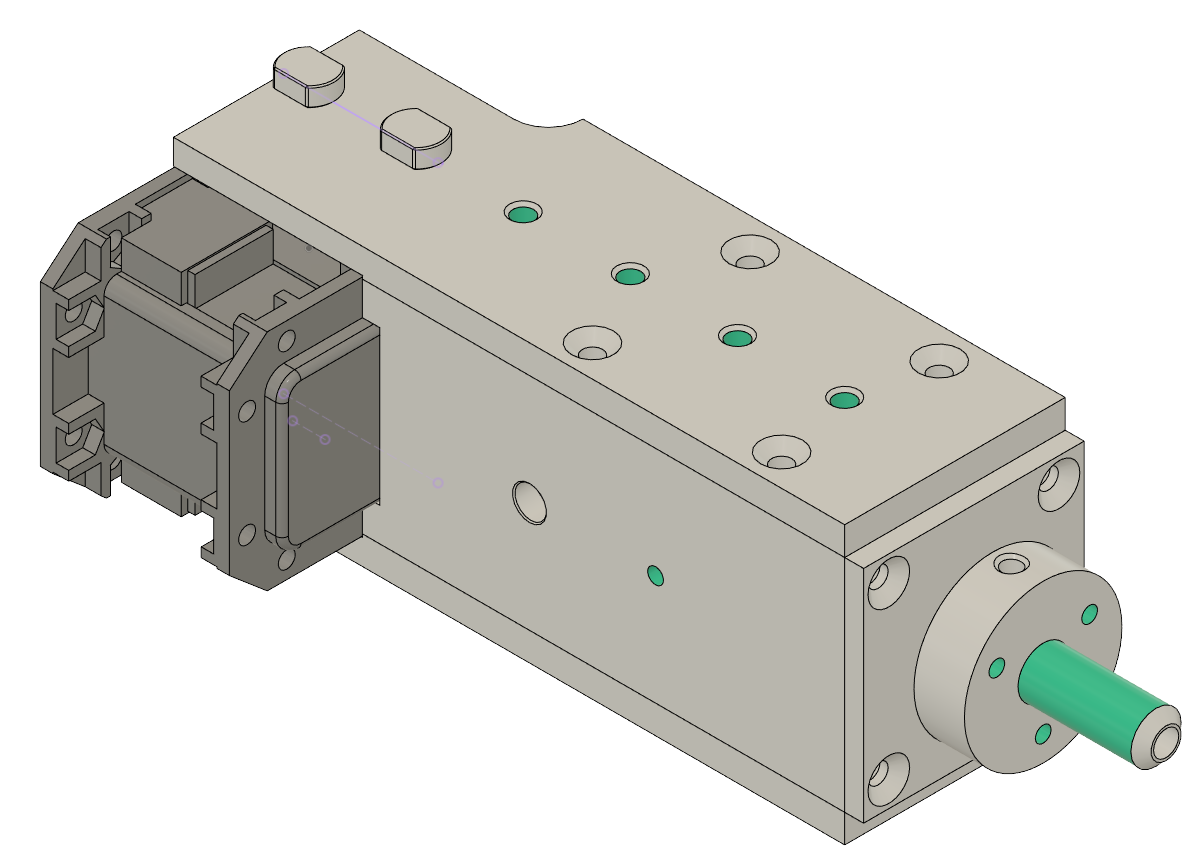
\includegraphics[height=6cm,width=1\textwidth,keepaspectratio]{motor_box v16_isometric_view.png}
            \label{fig:motor_box v16_isometric_view.png}
        \end{subfigure}
        \begin{subfigure}[c]{0.54\textwidth}
            \centering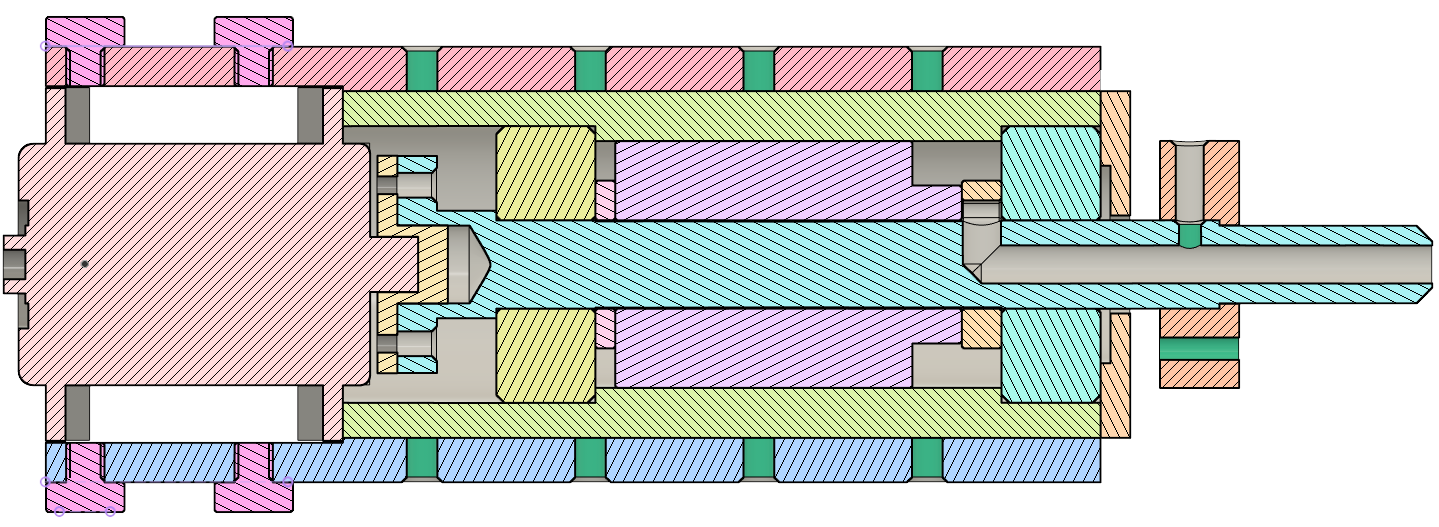
\includegraphics[height=6cm,width=1\textwidth,keepaspectratio]{motor_box v16_section_view.png}
            % \caption{capture2}
            \label{fig:motor_box v16_section_view.png}
        \end{subfigure}
    \end{figure}
\end{frame}

\begin{frame}[t]{Assembly drawing}
\framesubtitle{}
\vspace{-0.6cm}
\begin{figure}[H]
    \centering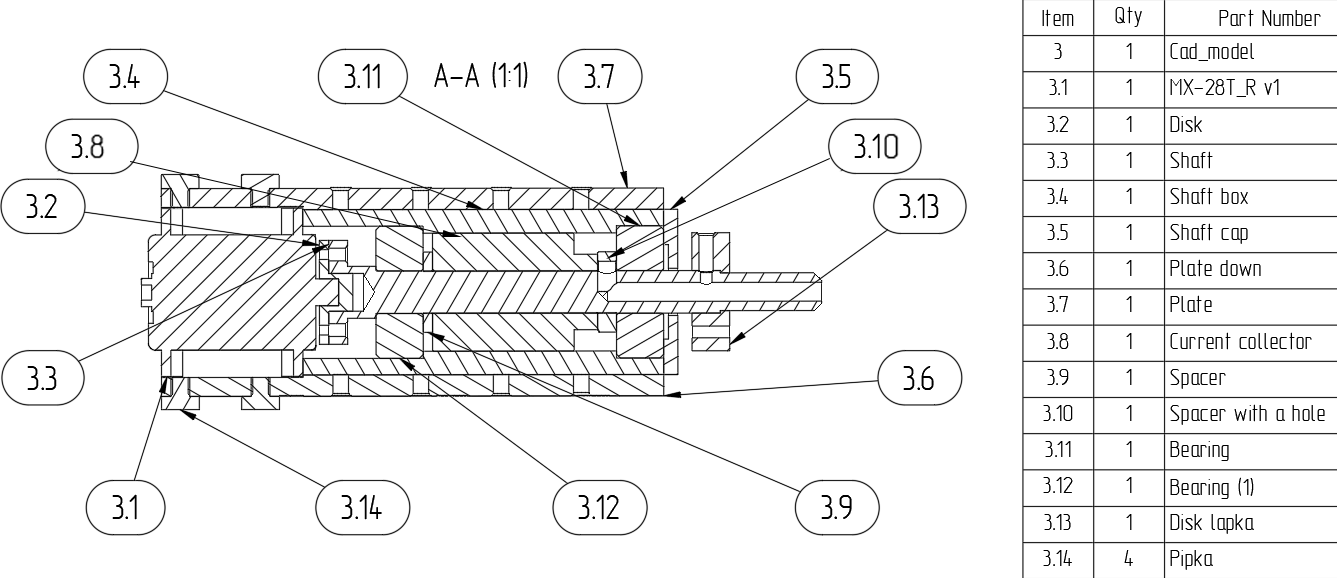
\includegraphics[height=6cm,width=1\textwidth,keepaspectratio]{parts.png}
    \label{fig:parts.png}
\end{figure}
\end{frame}

\fbckg{fibeamer/figs/last_page.png}
\frame[plain]{}

\end{document}